\chapter{Literature Review}
\label{Literature Review}

%/ INTRODUCTION
\section{Introduction}
Before looking into several researches which compares between reinforcement learning (RL) algorithms' advantages and disadvantages, preliminary lectures regarding RL implementations in trading are presented, to illustrate RL implementation in trading applications.

The first practical lecture \cite{LV90} aims to design an RL agent to perform spot trading. Here, the process starts with deciding how the data will be read and learned by an agent: either by reading the whole dataset, per-trade data chunks, per-window candles, or per-instrument. The next step is designing rewards. Reward and punishment design is deemed to be the core problem in trading and can be measured by different factors, e.g., profit and loss (PnL) on exit, per-period PnL, trend detection, and long hold prevention. It is also important to choose the features to extract from the data, for example, technical indicators, sentiment data; using different time resolutions are recommended. From there, the system is ready to be tested, using several possible instruments like trend curves, random walks, autocorrelation, etc. Lastly, a deep learning algorithm (see section \ref{sec:dl} is added to the system to improve learning capacity.

Results from this lecture show that RL may require huge amount of sample and is prone to overfitting, therefore results can vary among agents despite using the same code. Moreover, designing reward function is difficult: even with the assistance of trading indicators, it is difficult to avoid sticking to local optima. 

Another supporting lecture \cite{LV91} performs cryptocurrencies trading with the following qualities to measure: return-on-investment (ROI) and performance over market benchmarks. This research compares RL training in stationary and non-stationary data. Stationary data means that value distribution (mean, variance) at any time point is constant: one time point corresponds to one sample. Non-stationary data is the opposite: a series of data is considered as one individual sample. Since asset prices are non-stationary, the work mentions that conventional statistics and machine learning are not necessarily enough to tackle this problem. Therefore, the work uses REINFORCE, a policy gradient RL method that estimates the optimal policy by adjusting the policy that maximizes total reward. However, this algorithm is remarkably not sample efficient: old data are thrown away. Moreover, network parameters are prone to violently change, that explains the huge variability in training results.

\section{Deployment of Deep Reinforcement Learning and Market Sentiment Aware Strategies in Automated Stock Market Prediction} %41
Sagiraju and Mogalla \cite{LV41} compare several RL algorithms in predicting stock market in an automatic manner using both market price data and Twitter sentiment as the environment. The proposed framework is as shown in Fig. \ref{fig:lv4101}.

\begin{figure}[h]
    \centering
    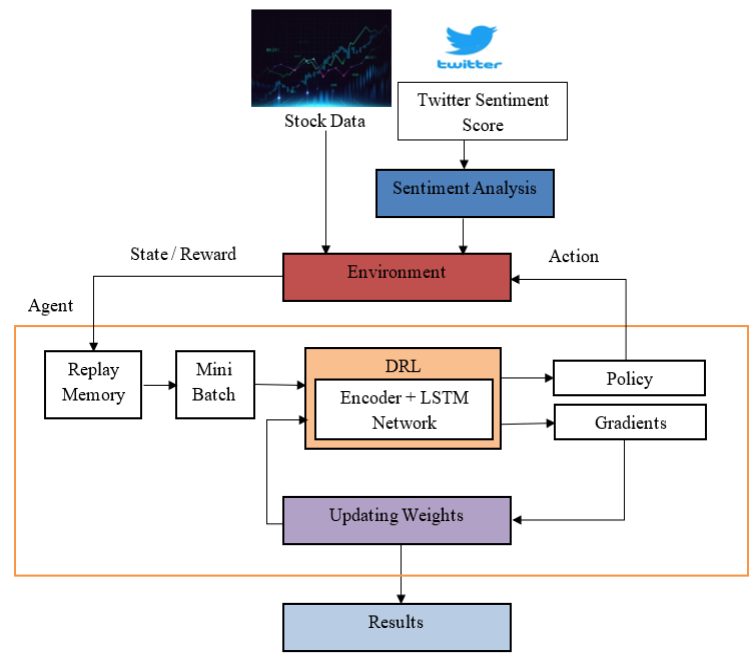
\includegraphics[width=0.55\textwidth]{graphics/2lv4101.png}
    \caption{Proposed framework by \cite{LV41}}
    \label{fig:lv4101}
\end{figure}

Various algorithms are compared: Deep Q-Networks (DQN), Deep Deterministic Policy Gradient (DDPG), Proximal Policy Optimization (PPO), Advantage Actor-Critic (A2C), and their proposed AutoEncoder-LSTM network combined with Reinforcement Learning (AE-LSTM+RL).

The daily closing data of Dow Jones Industrial Average (DJIA) and S\&P 500 data from 2006--2016 are used as training data, and are tested against the real data from 2016--2021. These data are combined with tweet sentiments in the range of [-1,1] calculated from engagement data. Yet, to align with the focus of this thesis, sentiment in this research is not discussed here.

Three benchmarks are used in evaluating the algorithms' performance: 
\begin{enumerate}
	\item Sharpe Ratio: $\frac{R_P-R_B}{\sigma_P}$, where $R_P$ = portfolio return, $R_B$ = benchmark rate, and $\sigma_P$ = standard deviation of portfolio. Penalizes any return below benchmark. Higher is better.
	\item Sortino Ratio: $\frac{R_P-R_B}{\sigma_D}$, where $R_P$ and $R_B$ are identical to above, and $\sigma_D$ = standard deviation of downside. Punishes returns below benchmark within a specific threshold. Higher is better.
	\item Maximum Drawdown (MDD): the maximum percentage of drawdown from the latest portfolio all-time high (ATH). Measures downside risk. Values closer to zero is better.
	\item Annual and cumulative portfolio return (ROI). Higher is better.
\end{enumerate}

The results show that, from the two assets' evaluation, AE-LSTM+RL returns the highest Sharpe Ratio and almost the best Sortino Ratio, annual ROI, and cumulative ROI, yet it causes the highest MDD. A2C performs slightly better or slightly worse to AE-LSTM+RL, PPO's results are often the worst in many benchmarks except it performs best at MDD, DQN and DDPG show similar results to A2C. Results can differ depending on the tested asset or time period, for example, PPO gives the highest annual DJIA return but by far the lowest cumulative return. Hence, supporting \cite{LV91}'s claim regarding the high variability between results given by RL tests, comparing and deciding which conventional algorithm performs the best is not a simple task.

\section{Deep Reinforcement Learning for Trading} %40
Similar to \cite{LV41} but excluding sentiments data and with different assets, Zhang et al. \cite{LV40} compare DQN, Policy Gradients (PG), A2C, with baseline algorithms Long Only, Sign(R), and Moving Average Convergence Divergence (MACD) using nine different metrics to maximize trading portfolio of five asset categories: commodity, equity index, fixed income, foreign exchange, and combined. From the results, DQN yields the best results in most metrics in every investment class except equity index. PG and A2C comparably perform worse than DQN but better than baseline algorithms, with A2C performs better than PG more often.

\section{A2C versus A3C} %compound
Espeholt et al. \cite{LV51} presents one comparison between A2C and A3C as a part of a larger comparison comprising of a proposed novel actor-critic algorithm, batched A2C, and A3C. The focus of the research is not related to trading but to find the most efficient algorithm to learn to complete two puzzles, measured by the training speed and learning outcome. The comparison between A2C and A3C is only found in the single-machine, GPU-less experiment, where A3C with 32 workers and 64 CPUs can process puzzle 1 and puzzle 2 at 6.5K and 9K frames per second (FPS). Meanwhile, batched A2C, 48 CPUs, with step synchronization, can reach 9K and 5K FPS, and batched A2C with trajectory synchronization yields 16K and 17.5K FPS. Again, this comparison is done using different settings and not mentioned in other parts of the study, hence cannot be easily concluded if A2C has any advantage over A3C.

Therefore, a qualitative comparison by Sewak \cite{LV52} between A2C and A3C will be included here. A3C is performed by distributing learning to multiple agents to be done in parallel. Each newly created agent copies the parameters from a centralized network parameter server and trains its data over the parameters. At one time, there will be a merge event where agents combine their own parameters with the global parameter, then replaces each's own parameters with the new global parameter to retrain. However, A3C's asynchronousness can be disadvantageous: agents may have different knowledge of the global state since not every agent pull the global parameters at one time. This is particularly bad if an agent fails or refuses to synchronize with the global parameters for a long time, causing training instability and slower convergence. A2C improves A3C by forcing agents to synchronize at specific times or conditions together at one time. Though, if an agent is unreachable or not responsive, this may cause synchronization delay.

\section{Verdict}
An extensive search of research repositories show that there has not been many, if any, research papers that explicitly compare between conventional algorithms, ML algorithms, and RL algorithms or between A2C against Asynchronous Advantage Actor-Critic (A3C), especially in the applications of trading and portfolio management. Moreover, the comparative results from different existing, or even within the same research, may wildly vary. With similar experiment settings and comparisons, the results can be different, see \cite{LV41} which shows that A2C yields the better results versus \cite{LV40} which clearly signifies that DQN is superior.
